\documentclass{standalone}
\usepackage{tikz}
\usepackage{verbatim}
\usetikzlibrary{positioning}
\begin{document}
\pagestyle{empty}
  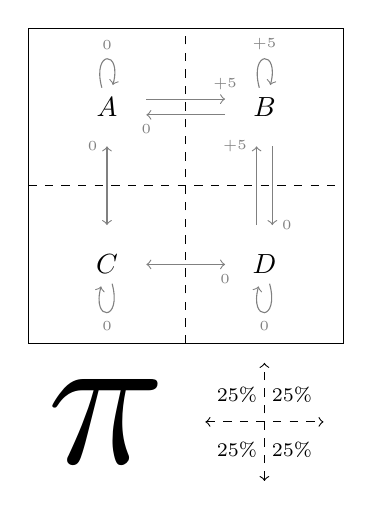
\begin{tikzpicture}
    \draw[step=2.0,black,thin, dashed] (0,0) grid (4, 4);
    \draw (0, 0) rectangle (4, 4);
    \node (a) at (1, 3) {$A$};
    \node (b) at (3, 3) {$B$};
    \node (c) at (1, 1) {$C$};
    \node (d) at (3, 1) {$D$};
    % States A-B
    \draw[->,gray] (1.5, 3.1) -- (2.5, 3.1) node[above, gray] {\tiny +5};
    \draw[->,gray] (2.5, 2.9) -- (1.5, 2.9) node[below, gray] {\tiny 0};
    % States B-D
    \draw[->,gray] (2.9, 1.5) -- (2.9, 2.5) node[left, gray] {\tiny +5};
    \draw[->,gray] (3.1, 2.5) -- (3.1, 1.5) node[right, gray] {\tiny 0};
    % States C-D
    \draw[<->,gray] (1.5, 1) -- (2.5, 1) node[below,gray] {\tiny 0};
    % States A-C
    \draw[<->,gray] (1, 1.5) -- (1, 2.5) node[left,gray] {\tiny 0};
    % Self-loops.
    \path[gray] (a) edge[loop above] node[above] {\tiny 0} (a);
    \path[gray] (b) edge[loop above] node[above] {\tiny +5} (b);
    \path[gray] (c) edge[loop below] node[below] {\tiny 0} (c);
    \path[gray] (d) edge[loop below] node[below] {\tiny 0} (d);
    % Policy
    \node at (1,-1) {\resizebox{1.5cm}{!}{$\pi$}};
    \draw[<->,dashed] (2.25, -1) -- (3.75, -1);
    \draw[<->,dashed] (3, -1.75) -- (3, -0.25);
    \node at (3.35, -0.65) {\scriptsize 25\%};
    \node at (2.65, -0.65) {\scriptsize 25\%};
    \node at (2.65, -1.35) {\scriptsize 25\%};
    \node at (3.35, -1.35) {\scriptsize 25\%};
  \end{tikzpicture}
\end{document}